\documentclass[a4paper]{article}
\usepackage[left=2cm,right=2cm,top=3cm,bottom=3cm]{geometry}
\usepackage[T1]{fontenc}
\usepackage{amsmath}
\usepackage{mathtools}
\usepackage{amssymb}
\usepackage{indentfirst}
\usepackage{graphicx}
\usepackage{algorithm}
\usepackage{algorithmic}
\usepackage{amsthm}

\graphicspath{ {./images/} }
\newtheorem{theorem}{Theorem}
\let\conjugate\overline


\title{\textbf{Pracownia z Analizy Numerycznej}\\{\Large Sprawozdanie do zadania P1.7}}
\author{Mateusz Leonowicz}

\begin{document}
\maketitle

\section{Wstęp}
    Wiele problemów w matematyce, fizyce czy informatyce sprowadzić można do wyznaczenia miejsc
    zerowych danego równania algebraicznego. Często nie wystarczy nam prosta analiza funkcji, a
    jedyne co możemy zrobić, to obliczenie jej wartości w danej, skończonej liczbie punktów jej dziedziny.
    Dlatego temat ten stał się jednym z fundamentalnych zagadnień analizy numerycznej, dzięki czemu
    powstało wiele metod iteracyjnych, które oczywiście mają swoje zalety i wady.
    
    \vspace{5mm}

    Celem tego sprawozdania jest przedstawienie metod obliczania pierwiastków wielomianów w postaci
    \[ax^3 + bx^2 + cx + d = 0 \qquad a, b, c, d \in \mathbb{R}\]
    które pozwalają komputerom na uzyskanie wyników z kontrolowanym błędem. Przedstawię trzy metody numeryczne oraz 
    rozwiązania z użyciem wzorów Cardano. Opiszę ich działadnie i charakterystykę, a następnie umieszczę ich porównanie
    razem z podsumowaniem.

    Wszystkie testy przeprowadzane będą z użyciem języka do analizy numerycznej Julia.
    
\tableofcontents

\newpage
\section{Metoda Newtona}
    Niech $f(x)$ będzie funkcją, której miejsce zerowe chcemy wyznaczyć. Niech $\alpha$ będzie takim zerem, a $x$
    jego przybliżeniem. Z twierdzenia Taylora, wiemy, że przybliżenie funkcji $f$, możemy zapisać w postaci:
    \[
        0 = f(\alpha) = f(x + e) = f(x) + ef'(x) + \frac{f''(\xi)}{2!}e^2 \qquad \xi \in \text{interv}(x, \alpha) 
    \tag{1}\]

    Jeśli nasz wyraz $\frac{f''(\xi)}{2!}e^2$ będzie dostatecznie mały, to możemy go pominąć i rozwiązać równanie 
    względem $e$, co daje nam:
    \[
        e = \frac{-f(x)}{f'(x)}  
    \]

    Jeśli $x$ jest dostatecznie dobrym przybliżeniem $\alpha$, to $x - e$ będzie jeszcze lepszym przybliżeniem tego
    pierwiastka. Na tej różnicy opiera się metoda Newtona, która po wybraniu startowego przybliżenia $x_0$ zera $\alpha$
    polega na stosowaniu rekurencyjnego wzoru:
    \[
        x_{n+1} = x_n - \frac{f(x)}{f'(x)} \qquad n \geq 0
    \tag{2}\]

    Dobranie startowego punktu $x_0$ w tej metodzie jest bardzo istotne, gdyż metoda Newtona nie zawsze jest zbieżna.
    Jeśli dobierzemy odpowiednio punkt początkowy będziemy mieli zbieżność kwadratową, z wyjątkiem przypadków, gdy 
    istnieją wielokrotne zera funkcji. Wtedy otrzymamy zbieżność liniową.

    \vspace{5mm}

    Metoda Newtona opiera się na linearyzacji funkcji $f$, co pozwala nam na dobre przybliżanie wartości funkcji w małym
    otoczeniu punktu $x$. Możemy więc rozumieć tę metodę, jako przybliżanie miejsc zerowych funkcji za pomocą jej stycznych,
    co oczywiście niesie za sobą groźbę rozbieżności.

    \vspace{10mm}

    \begin{figure}[h]
        \centering
        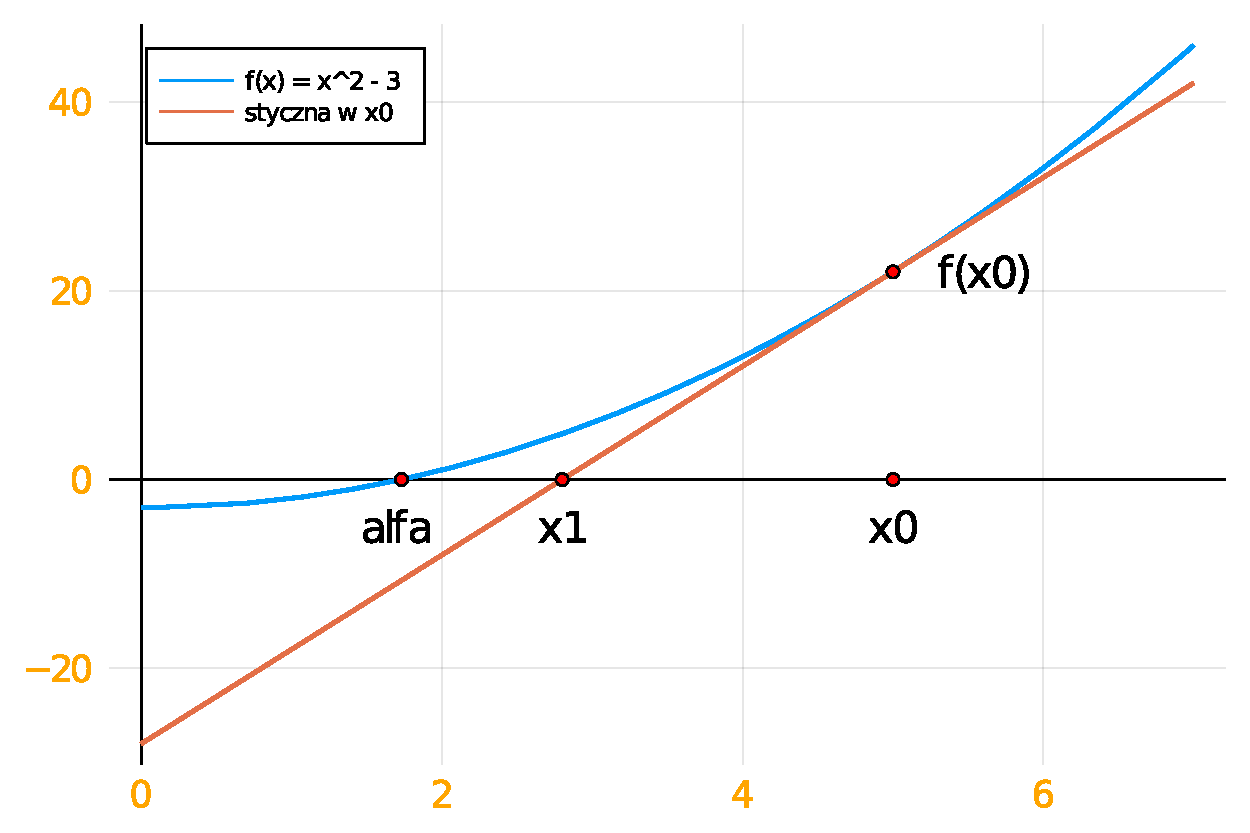
\includegraphics[width=12cm]{newtonPlot}
        \caption{Interpretacja geometryczna metody Netwona}
    \end{figure}

\newpage
\section{Metoda biskecji}
    Niech $f$ będzie funkcją ciągłą w przedziale $[a,b]$ i jeśli $f(a)f(b) < 0$, czyli funkcja zmienia znak na końcach przedziałów, to
    ta funkcja musi mieć zero w przedziale $(a,b)$ i jest to oczywiście konsekwencja twierdzenia Darboux. Możemy więc zmniejszyć nasz
    przedział o połowę wybierając punkt $c$, taki że $f(c)f(a) < 0$ lub $f(c)f(b) < 0$. Uzyskaliśmy nowy przedział, w którym wiemy, że
    znajduje się nasze miejsce zerowe. Na tym rozumowaniu opiera się metoda biskecji, którą wyrazić można następującym algorytmem:

    \begin{algorithm}
    \caption{Szukanie pierwiastka funkcji $f$}
    \begin{algorithmic}
    \REQUIRE $\epsilon\ a_0\ b_0\ M \quad \text{takie, że} \quad f(a_0)f(b_0) < 0$
        \STATE $n \leftarrow 1$
        \STATE $left \leftarrow a_0$
        \STATE $right \leftarrow b_0$
        \WHILE{$n < M$}
        \STATE $c = \frac{left + right}{2}$
        \IF{$f(c) = 0 \vee \lvert left - right \lvert < \epsilon$}
        \STATE $\text{pierwiastkiem jest}\ c$
        \ELSE
        \STATE $n \leftarrow n + 1$
        \ENDIF
        \IF{$f(left)f(c) < 0$}
        \STATE $left \leftarrow c$
        \ELSE
        \STATE $right \leftarrow c$
        \ENDIF
        \ENDWHILE
        \end{algorithmic}
    \end{algorithm}

    Algorytm uwzględnia trzy kryteria zakończenia obliczeń, ponieważ inaczej istniałoby
    ryzyko zapętlenia. Pierwszym jest oczywiście znalezienie takiego punkt $c$, że $f(c) = 0$. Drugim z nich jest 
    skończona liczba iteracji wyrażona zmienną $M$. Oprócz tego, obliczenia są przerywane, 
    jeżeli błąd jest dostatecznie mały, tj. mniejszy od $\epsilon$. Łatwo znaleźć przykłady funkcji w których
    brak któregoś z kryterów mógłby prowadzić do bardzo błędnych wyników.

    \begin{figure}[h]
        \centering
        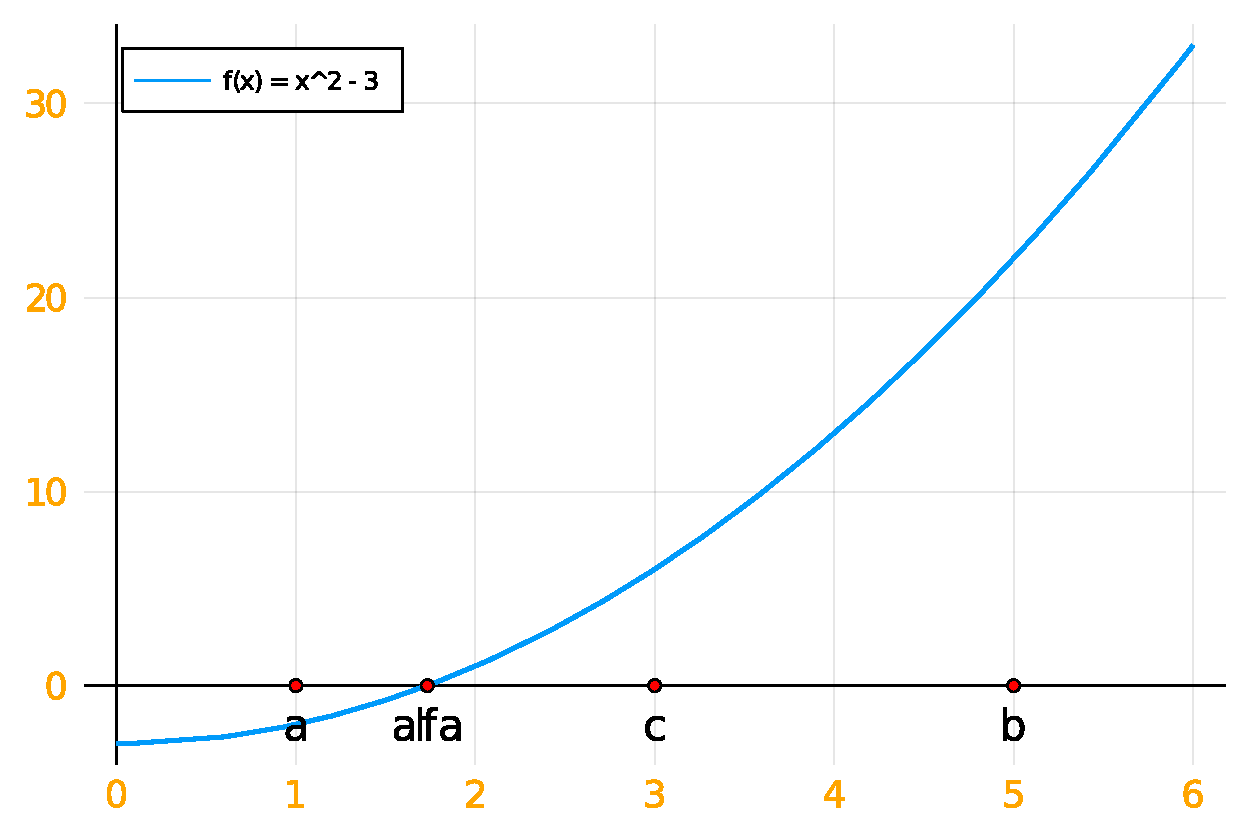
\includegraphics[width=12cm]{bisectionPlot}
        \caption{Interpretacja geometryczna metody bisekcji}
    \end{figure}

\newpage
\section{Metoda Bairstowa}
    Wymienione metody do tej pory, oprócz oczywistych problemów z wybraniem początkowych wyrazów, czy niejednolitą zbieżnością, mają
    jedną o wiele poważniejszą dla nas wadę. W ich akutalnej postaci, jeśli nasza funkcja $f$ będzie miała pierwiastki zespolone, to
    ich nie wyznaczymy. Do tego potrzebujemy bardziej zaawansowanego i ogólnego algorytmu. Najpierw przedstawię 
    kilka letmatów, które przydadzą się do wyprowadzenia metody Bairstowa.
    \begin{theorem}
        Wielomian stopnia n ma dokładnie n pierwiastków w przestrzeni zespolonej, gdy każdy z nich liczony jest tyle razy, ile wynosi jego krotność.
    \end{theorem}
    
    \begin{theorem}
        Jeśli wielomian $w(x)$ stopnia $n \in \mathbb{N}$ ma współczynniki 
        $a_i \in \mathbb{R},\ 0 \leq i \leq n$, oraz $\alpha \in \mathbb{C} \setminus \mathbb{R}$ jest jego 
        miejscem zerowym, to $\conjugate{\alpha}$ też jest jego miejscem zerowym, a iloczyn
        kwadratowy $(x - \alpha)(x - \conjugate{\alpha})$ dzieli bez reszty wielomian $w(x)$.
    \end{theorem}
    \begin{proof}
        Mamy wielomian $w(x) = a_{n}x^n + a_{n-1}x^{n-1} + \ldots + a_{0}x^0$, oraz z założenia wiemy, że
        $w(\alpha) = 0$. Korzystając z dwóch własności sprzężenia $\conjugate{x + y} = \conjugate{x} + \conjugate{y}$,
        ${\conjugate{xy} = \conjugate{x}\conjugate{y}}$ otrzymujemy wprost równość: $w(\conjugate{\alpha})$. Ponieważ
        $\alpha$ jest pierwiastkiem nierzeczywistym, to $\alpha \neq \conjugate{\alpha}$. Z twierdzenia o reszcie, wynika, że
        iloczyn $(x - \alpha)(x - \conjugate{\alpha})$ dzieli nasz wielomian bez reszty.
    \end{proof}

    \begin{theorem}
        Dzielenie wielomianu 
        \[
            w(x) = a_{n}x^n + a_{n-1}x^{n-1} + \ldots + a_{0}x^0
        \]
        Przez wielomian w postaci $(x^2 - ux - v) \ \ u,v \in \mathbb{C}$ daje iloraz i resztę równe:
        \[
            \begin{array}{c}
                \phi(x) = b_{n}x^{n-2} + b_{n-1}x^{n-3} + \ldots + b_{2}x^0 \\
                r(x) = b_{1}(z - u) + b_{0}
            \end{array}
        \]
        Których współczynniki dane są rekurencyjnym wzorem:
        \[
            b_{n+1} = b_{n+2} = 0, \qquad b_k = a_k + ub_{k+1} + vb_{k+2} \qquad (n \leq k \leq 0).  
        \tag{3}\]
        Dowód jest dość prosty i polega na porównaniu współczynników po obu stronach równania:
        \[
            w(x) = \phi(x)(x^2 - ux - v) + r(x)  
        \]
    \end{theorem}

    Dla każdego wielomianu $w$ stopnia $n \leq 2$ znajdziemy więc takie $u$ i $v$, że nasz wielomian $(x^2 - ux -v)$ będzie dzielił
    $w$ bez reszty. Na szukaniu tych rzeczywistych czynników opiera się metoda Bairstowa. W $r(x)$ nasze współczynniki $b_0$ i $b_1$
    zależą od $u$ i $v$, więc zapiszmy:
    \[
        b_0(u, v) = 0 \qquad b_1(u, v) = 0  
    \]
    Są to równania nieliniowe, dwuargumentowe. Szukamy więc takich poprawek oznaczonych $\delta u$ i $\delta v$, które spełniałyby równanie:
    \[
        b_0(u + \delta u, v + \delta v) = b_1(u + \delta u, v + \delta v) = 0  
    \]
    Z twierdzenia Taylora możemy zlinearyzować jedną z powyższych równości, co daje:
    \[
        \begin{array}{c}
            b_0(u, v) + \frac{\partial b_0}{\partial u}\delta u + \frac{\partial b_0}{\partial v}\delta v = 0  \\\\
            b_1(u, v) + \frac{\partial b_1}{\partial u}\delta u + \frac{\partial b_1}{\partial v}\delta v = 0  
        \end{array}
    \tag{4}\]
    Zdefiniujmy więc wyrazy pomocnicze, które oczywiście spełniają rekurencyjną zależność z (3):
    \[
        c_k = \frac{\partial b_k}{\partial u} \qquad d_k = \frac{\partial b_{k-1}}{\partial v} \qquad (0 \leq k \leq n) 
    \]
    Podstawiając do równań z (4) i uzależniając równania od $\delta v$ i $\delta u$ otrzymujemy:
    \[
        \begin{array}{c}
            \delta u = (c_1b_1 - c_2b_0)\frac{1}{J} \\\\
            \delta v = (c_1b_0 - c_0b_1)\frac{1}{J} \\\\
            J = c_0c_2 - c_1^2
        \end{array}
    \]
    Otrzymaliśmy więc wzór na lepsze przybliżenie naszej pary $(u, v)$.

\end{document}
